\chapter{Cyfrowy system wizyjny}
\label{cha:csw}
%TODO mało inforamtywny tytuł.

%TODO Kilka zdań o zawratości rozdziału - szczególnie, że jest różnorodna.

%TODO Jak tam na to patrzę, to może być to podzielić dwa rozdziały:
%TODO podczerwień, kamery, kalibracja itp.
%TODO detekcja osób

\section{Podczerwień}

Mianem podczerwieni określa się promieniowanie elektromagnetyczne w zakresie fali o długości od 0,75 $\mu m$ do 1000~$\mu m$.
Każde ciało które ma temperaturę wyższą niż zero absolutne emituje swoją powierzchnią promieniowanie. 
Im większa jest temperatura ciała tym więcej promieniowania emituje. %TODO wyższa + powt. emituje
Dla każdej temperatury danego ciała istnieje charakterystyczna długość fali o najwyższej wartości mocy promieniowania. 
Wraz z wzrostem temperatury ta częstotliwość przesuwa się w zakres fal widzialnych. 
Można to zaobserwować, gdy stal osiąga wysoką temperaturę co skutkuję emisją światła. 

%TODO Tu by się przydało jakieś zdanie łączące, bo tak to się pojawia ni z gruchy...
Ciało doskonale czarne całkowicie pochłania padające na nie promieniowanie oraz emituję promieniowanie ściśle związane z jego temperaturą. 
Wykres na rysunku \ref{fig:perfect_black} przedstawia tą charakterystykę. 
Promieniowanie podczerwone jest częściowo pochłaniane przez atmosferę ziemską . 
Na rysunku \ref{fig:atmosfera_int} przedstawiono  tzw. transmisyjność atmosfery. 
W aparaturze rejestrującej w podczerwieni wykorzystuję się dwa zakresy przy których transmisyjność jest największa: 3 -- 5 $\mu m$ (MIWR, ang. \textit{mid wave infrared} -- podczerwień fal średnich) oraz 8 -- 14 $\mu m$ (LWIR , ang. \textit{long wave infrared} -- podczerwień fal długich)\cite{niklaus2007mems}.

\begin{figure}
\centering
\includegraphics[width=0.8\linewidth]{images/Atmosfaerisk_spredning}
\caption[Wykres transmisyjności atmosfery dla promieniowania podczerwonego ]{Wykres transmisyjności atmosfery dla promieniowania podczerwonego \cite{wiki:infrared}.}
\label{fig:perfect_black}
\end{figure}

\begin{figure}
\centering
\includegraphics[width=0.4\linewidth]{images/perfect_black_emi}
\caption[Emisyjność ciała idealnie czarnego]{Emisyjność ciała idealnie czarnego.}
\label{fig:atmosfera_int}
\end{figure}

%TODO Tu by się przydało coś o kamerach termowizyjnych napisać, albo nawet o kamerach wizyjnych i termowizyjnych, a dopiero potem o ich łączeniu.

\section{Metody akwizycji obrazu}
%TODO trzeba zmienić ten tytuł...

Większość implementacji wykorzystuje układ dwóch równoległych do siebie kamer, której przykład przedstawia rysunek \ref{dual_camera}.  %TODO tu trzeba napisać jawnie jakie to są kamery 
%TODO dlaczego od razu przejście do stereo
Często obrazy z kamer różnią się, wynika to z ich budowy, różnej rozdzielczości, kąta widzenia jak oraz zniekształceń soczewkowych.
Do poprawnego odwzorowania tej samej sceny w obu widmach należy zastosować algorytm mający na celu dopasowanie obu obrazów.
%TODO (tj. ..... /napisać co to jest dopasowanie/)

Pierwszym z etapów poprawnego dopasowania obrazów jest kalibracja.
Wykonuje się ją z~wykorzystaniem specjalnych plansz, które pozwalają określić położenie pewnych punktów w przestrzeni w obu rejestrowanych zakresach promieniowania. 
Punkty te pozwalają na obliczenie relacji między obrazami. 
Plansze mogą być aktywne (posiadają własne źródło ciepła) albo pasywne (przesłaniają obce źródło ciepła). 
W równoległym układzie kamer występuje również zjawisko paralaksy, które powiększa się wraz z wzrostem odległości obiektu od punktu kalibracji. 
W pracy \cite{hwang2015multispectral} autorzy zastosowali zwierciadło półprzezroczyste wykonane z wafla krzemowego pokrytego cynkiem do rozdzielenia obrazu w celu eliminacji tej wady (rysunek \ref{multispectral}).
%TODO Ten rysunek 2.3 b) jest jakiś nieczytelny i wymaga opisu/komentarza.

\begin{figure}[h]
\centering
\begin{subfigure}{0.45\textwidth}
\centering
\includegraphics[width=1\textwidth]{images/dual-camera}
\subcaption{\label{dual_camera}}
\end{subfigure}
\begin{subfigure}{0.45\textwidth}
\centering
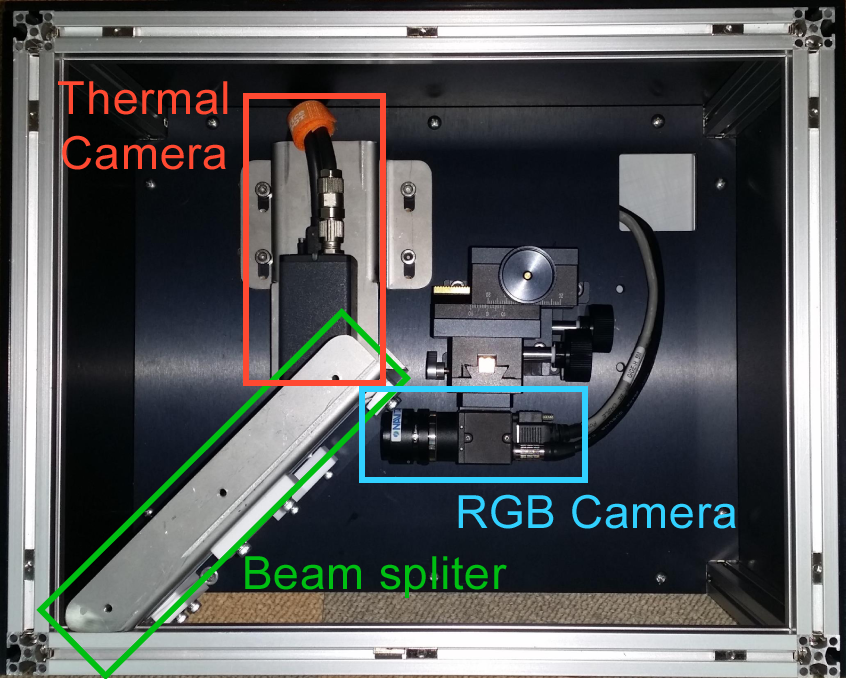
\includegraphics[width=1\textwidth]{images/multispectral}
\subcaption{\label{multispectral}}
\end{subfigure}
\caption{\label{fig:cameras_systems}Sposoby akwizycji obrazów: \protect\subref{dual_camera} dwie kamery równolegle \cite{lee2015robust}, \protect\subref{multispectral} z wykorzystaniem zwierciadła półprzezroczystego \cite{hwang2015multispectral}.}
\end{figure}


\section{Model geometryczny}
%TODO To chyba powinien być podrozdział - bo to jest wszczegółowienie tego ogólnego modelu integracji kamer.

Do opisu matematycznego systemu wykorzystuje się model kamery otworkowej. 
Dzięki niemu można opisać relację między trójwymiarową przestrzenią, a dwuwymiarowym obrazem za pomocą projekcji perspektywicznych. %TODO chyba perspektywicznej (projekcja jest jedna)
Nie stanowi on najdokładniejszego opisu matematycznego kamery, nie ma w nim uwzględnionych zakłóceń soczewkowych, dobre rezultaty w wielu aplikacjach.  %TODO czegoś brakuje np. jednakże  zapewnie dobre
Składa się ona z 2 zestawów parametrów: zewnętrznych oraz wewnętrznych.
%TODO Co to jest "ona" ale chyba trzeba już po prostu napisać Model, czy Transformacja
Parametry zewnętrzne definiują lokację kamery względem zewnętrznego układu współrzędnych. 
Są reprezentowane przez wektor translacji \(T\) między układem związanym z kamerą \( \left ( X_{c},Y_{c},Z_{c}\right ) \),
a zewnętrznym \(\left ( X,Y,Z\right )\). 
Drugim parametrem jest macierz rotacji \( R \) (między osiami tych dwóch układów).
Punkt \(P = \left [ X,Y,Z \right ]^T \) będący w zewnętrznym układzie współrzędnym ma swój odpowiednik w układzie wewnętrznym, który można określić zależnością 

\begin{equation}
P_{c} = RP+T
\end{equation}

Właściwości optyczne kamery można przedstawić w postaci macierzy kamery.
\begin{equation}
K = \begin{bmatrix}
f_x & 0 & x_0 \\ 
0 & f_y & y_0\\ 
0 &0 & 1
\end{bmatrix}
\end{equation}
gdzie:
\begin{conditions}
f_{x}, f_{y} & ogniskowa kamery wyrażona w liczbie pikseli, \\
x_{0},y_{0} & współrzędne punktu głównego. 
\end{conditions}

Macierz $K$ określa związek między znormalizowanymi współrzędnymi w układzie odniesienia kamery danych wzorem \(x_n = \frac{X_c}{Z_c}, y_n = \frac{Y_c}{Z_c}\), a~odpowiadającym im współrzędnymi punktów na obrazie \(u,v\):

\begin{equation}
\begin{bmatrix}
u \\
v \\
1
\end{bmatrix} = K \begin{bmatrix}
x_n \\
y_n \\
1
\end{bmatrix}
\end{equation}

%TODO To jest wszystko OK, ale nie ma tutaj wprost powiedziane jak dopasować dwa obrazy. Może jakiś przykład, ilustracja itp. Ogólnie omówienie jak wykonać taką kalibrację.


%TODO Osobny rozdział ....
\section{Algorytmy detekcji pieszych}

W cyfrowej analizie obrazu rozpoznawanie pieszych jest jedną z najbardziej aktywnie rozwijanych dziedzin. 
W przeciągu kilkudziesięciu lat powstało ponad tysiąc artykułów poruszających to zagadnienie \cite{zhang2015filtered}, w~których zaproponowano wiele różnych metod. 
Większość metod opiera się o analizę obrazu tylko w jednym spektrum: widzialnym albo podczerwieni. 
Praca \cite{hwang2015multispectral} pokazała że połączenie obu obrazów może dać lepsze wyniki. 
Podobnie w artykule \cite{gonzalez2016pedestrian} wykazano, że analiza multispektralna jest skuteczniejsza w dzień niż w nocy (o około 5\% AMR (ang. \textit{avrange miss rate}). 
W artykule \cite{benenson2014ten} autorzy podsumowują osiągnięcia w dziedzinie detekcji pieszych w latach 2004 -- 2014. 
Wyróżniono ponad 40 różnych podejść do problemu. 
Artykuł jest oparty o bazę danych Caltech-USA, która zawiera obrazy w~kolorze. %TODO Eksperymenty w artykule.... 
Jednym z wniosków jest, że przez ostanie dziesięć lat największy postęp został osiągnięty głównie dzięki dopracowaniu cech, które są wyodrębniane z obrazu niż ulepszanie klasyfikatora. 
Dodatkowo autorzy połączyli cechy dające najlepsze wyniki i stworzyli własną metodę która uzyska 12\% zysk AMR względem najlepszej badanej wcześniej metody.

%TODO a coś o głębokich sieciach ? Jakoś pominął Pan ten temat.

Dla typowego algorytmu detekcji pieszych można wyróżnić trzy podstawowe etapy:

\subsection{Ustalenie regionu zainteresowań} 

Jest to obszar zwany ROI (ang. \textit{region of interest}), w którym potencjalnie mogą znajdować się piesi. 
Wiele podejść uznaje cały obraz jako ROI i stosuje okno przesuwne sprawdzając każdy możliwy fragment obrazu. 
Jeżeli scena jest rejestrowana przez nieruchomą kamerę, ROI można określić poprzez różnicę między zapamiętanym tłem, a aktualnym obrazem (tzn. modelowanie i~odejmowanie tła). 
Wyodrębnienie ROI jest bardzo istotne w przypadku pracy w czasie rzeczywistym, ze względu na ograniczony czas analizy pojedynczego obrazu.

%TODO A jakieś inne metody wyodrębniania ROI

\subsection{Wyodrębnienie cech}

Do najbardziej popularnych cech można zaliczyć:

\begin{enumerate}
%TODO proszę to sprawdzić, bo zmieniłem gramatykę.
\item Histogramy zorientowanych gradientów (HOG). %TODO ang. skrót
Algorytm został zaproponowany przez N.Dalala i B. Triggs w pracy \cite{dalal2005histograms} i~stał się jednym z najbardziej popularnych technik w dziedzinie rozpoznawania ludzi. %TODO nie rozpozawania, tylko detekcji
Jest cały czas rozwijany i modyfikowany w wielu pracach naukowych.
Technika polega na zliczeniu kierunków gradientów, uzyskanych z 2 masek kierunkowych \(\begin{bmatrix}-1 & 0 & 1\end{bmatrix} \) i \( \begin{bmatrix}-1 & 0 & 1 \end{bmatrix}^T\), w komórkach o określonych wymiarach. 
Komórki te są organizowane w bloki, w obrębie których następuje normalizacja. 
Wektorem cech jest połączenie wszystkich histogramów z wszystkich bloków w jeden wektor.

%TODO Ciut więcej detali o tej metodzie (interpolacja, po co normalizacja itp.)

\item Lokalne wzorce binarne LBP (ang. \textit{Local Binary Paterns}).
Oryginalnie deskryptory te zaproponowane zostały do opisu tekstur. %TODO \cite też coś ojala 
Analizowany obraz zostaje podzielony na bloki. 
Następnie, do każdego piksela w bloku zostaje przypisany wzorzec binarny na podstawie wartości pikseli w jego sąsiedztwie. 
Jeżeli wartość sąsiadującego piksela jest większa od centralnego to przyjmuje on wartość 1. 
%TODO Tu coś dodac, że w ten sposobó...
Następnie zostaje obliczony histogram dla każdego bloku. 
Histogramy z wszystkich bloków wchodzących w skład obrazu tworzą wektor cech \cite{ojala2002multiresolution}.

\item Falki Haara.
Określają różnicę w kontraście między dwoma przylegającymi prostokątnymi obszarami. 
Są łatwe do skalowania i nie wymagają dużych nakładów obliczeniowych.

%TODO coś więcej

\item Kolor. W analizie obrazów wykorzystuje różne przestrzenie barw np. RGB, HSV oraz LUV.
%TODO też coś więcej. 

\item Lokalne struktury. W odróżnieniu od pojedynczych pikseli można wyznaczyć lokalne struktury o podobnym kolorze. (np. głowa i ręce mają podobne kolory, jednolita koszula, spodnie).
%TODO też coś więcej. Na jakiej zasadzie się ich używa.


\end{enumerate}

\subsection{Klasyfikator}
Otrzymany wektor cech jest poddany klasyfikacji, której wynik decyduje czy obraz zawiera człowieka.
W pracy \cite{benenson2014ten} autorzy wyróżnili 3 dominujące rodziny metod:

\begin{enumerate}
\item Rodzina DPM (ang. Deformable Part Detectors) ??? wykrywacze deformowlnych elementów ???. %TODO a nie Deformable Part Model ?
Technika polega na klasyfikacji poszczególnych elementów człowieka (głowa, tułów, nogi). Następnie jest analizowany układ tych elementów na obrazie i podjęcie decyzji o obecności człowieka.
%TODO ale ogólnie to prosze doczytać.

\item Deep networks – głębokie sieci neuronowe.

\item Decision forests – ?? lasy decyzyjne ?? zbiór nieskorelowanych drzew decyzyjnych.

\item inne: SVM (ang. support vector machine – maszyna wektorów nośnych), AdaBoost itp.


%TODO Też trzeba rozbudować ten opis. Poza tym te sieci głębokie to trzeba by omówić osobno.

\end{enumerate}

%TODO Nie omówił Pan specyfiki detekcji w podczerwieni.

%TODO Po tym ogólnym omówieniu oczekwiałbym bym jednak szegółowego omówienia publikacji. Najbardziej zależy mi na 4 z Poznania (nie wiem czy Panu podsyłąłem - mogę to zrobić.) Poza tym ma Pan tam kilka publikacji we wstepnie, o tej fuzji - może coś z tego. Opiać też metodę z inzynierki itp.




%TODO To chyba też osobny rodział. Powinien on zacząć się od omówienie technologii FPGA, Zynq i wykorzystywanej platformy sprzętowej.

\section{Wykorzystanie FPGA w analizie obrazu}

Tradycyjne systemy wizyjne zwykle bazują na architekturze sekwencyjnej.
W tym rozwiązaniu obraz jest sukcesywnie poddawany kolejnym przekształceniom, a~wyniki pośrednie zapisywane są w pamięci operacyjnej. 
W aplikacji procesorowej operacje te są wykonywane przez układ arytmetyczno-logiczny. 
Kolejne kroki algorytmu są kompilowane w ciąg instrukcji dla procesora ,który oprócz operacji matematycznych dużą część pracy poświęca na pobieranie i dekodowanie rozkazów oraz na odczytywanie i zapisywanie danych do pamięci. 
By taka aplikacja mogła pracować w czasie rzeczywistym, cała procedura musi wykonać się szybciej niż przychodzące dane obrazu, co wymusza wysokie taktowanie procesora sięgające kilku GHz. 
%TODO dodać, że to i tak nie zawsze pomaga. Poza tym wypada jakoś skomentować fakt istnienie procesorów wielordzeniowych.

W przypadku podejścia równoległego, implementacja poszczególnych kroków algorytmu odbywa się w osobnych procesach. 
Jeżeli kolejne kroki algorytmu wymagałyby danych otrzymanych z poprzednich, to zysk takiego zabiegu byłby równy zero. %TODO to jest dość niejednoznaczne. Musi Pan to opatrzyć jakimś lepszym komentarzem/przykładem.
By uzyskać znacznie przyspieszenie algorytm musi mieć możliwość podzielenia na wiele niezależnych części. 
Maksymalne do uzyskania przyspieszenie jest określone przez prawo Amdahla: 
\begin{equation}
P_w =\frac{1}{ s + \frac{1-s}{n_w}}
\end{equation}
gdzie:
\begin{conditions}
P_{w} & przyspieszenie algorytmu w systemie wieloprocesorowym, \\
s & cześć algorytmu niepodlegająca zrównolegleniu (wartość od zera do jeden), \\
n_{w} & liczba elementów obliczeniowych.
\end{conditions}

Teoretycznie jedynym ograniczaniem w możliwości zrównoleglenia obliczeń jest liczba zasobów dostępnych, jednak istotnym aspektem jest sposób dostarczania danych do zaimplementowanych w układzie procesorów. %TODO procesorów, czy modułów obliczeniowych - no bo w sumie to musi się Pan ogólnie zdecydować, czy pisze to Pan ogólnie, czy z uzględnieniem architektury.
Czas i przepustowość jaka jest potrzebna do odczytania i zapisu obrazu po przetworzeniu z i do pamięci jest najczęściej wąskim gardłem systemu wizyjnego. %TODO to z i do źle wygląda
Z tego powodu przetwarzanie obrazu bezpośrednio z sensora w czasie jego akwizycji jest chętnie wykorzystywane, gdyż zmniejsza to liczbę operacji odczytu i zapisu. \cite{garcia2014survey}

%TODO No i w ten sposób to Pan w rodziale o FPGA, ani razu nie użył słowa FPGA.
%TODO Druga sprawa to jest GPU - tez się tu powinno pojawić.


%TODO To trzeba wkomponować w rozdział o algorytmach. Ew. rozdział FPGA można dać przed algorytmy i wtedy omówić metody programowe oraz sprzętowe.
\section{Przegląd literatury}

\subsection{Podobne rozwiązania}
%TODO ponieważ te opisy są dość obszerne proszę jednak dać to w osobne podrozdziały subsub (czy jak to wyjdzie)

W pracy \cite{kolzpoz} autorzy opracowali algorytm pozwalający na szybką i efektywną detekcję przechodniów w czasie rzeczywistym. 
Termowizja pozwala na uzyskanie dobrego kontrastu między poszukiwanym przechodniem a otoczeniem. 
System dedykowany jest do pracy w nocy, kiedy kontrast między człowiekiem pozwala na jednoznaczne ich rozróżnienie.  %TODO między człowiekiem, a czym ?
Rozwiązanie bazuje na ulepszonym algorytmie progowania i segmentacji obrazu. 

Pierwszym etapem jest wyodrębnienie obszarów zainteresowań (ROI). 
Pozwala to na znaczne ograniczenie obszaru obrazu do analizy. %TODO rozmiaru analizowanych fragmentów obrazu (czy jakoś tak)
Obraz w odcieniach szarości zostaję poddany binaryzacji z użyciem dwóch progów: mniejszym i większym. 
Dodatkowo każdy wykryty obszar tworzy dodatkowy ROI przylegający do pierwotnego. %TODO 1. powt. dod, 2. niejasen
Progowanie z pojedynczym progiem jest niewystarczające w wielu wypadach dlatego autorzy zastosowali podwójne progowanie. %TODO ale to już Pan napisał wcześniej.
Pozwala to na detekcję przechodniów w różnych rejonach obrazu o różnym kontraście. 
Progi zmieniają się wraz z dynamiką obrazu wejściowego. 
%TODO Proszę to kwestię dwóch progów lepiej opisać. Bo nie wiadomo jak co i po co jest robione.
W obrazie termicznym człowieka często występuję obszar o niższej temperaturze w okolicach bioder. 
Skutkuje to przerwą w zbinaryzowanym obiekcie i błędną klasyfikację np.: samych nóg. 
Autorzy opracowali technikę polegającą na powiększeniu obszaru. 
Łączy ona dwie połówki człowieka, jeżeli posiadają one wspólne współrzędne wzdłuż pionowej osi tworząc nowy obszar. %TODO to "tworząc" coś nie pasuje
Ostatecznie obie grupy obszarów zainteresowania uzyskanych z obu progowań zostają połączone. %TODO to też jest niejasne. 

Następnym krokiem jest filtracja wyników. 
Ma ona na celu zredukowanie liczby obszarów przed końcową analizą. 
Autorzy zastosowali filtrację opierającą się na proporcji obszaru zainteresowań. 
Pozytywnie zakwalifikowane zostały tylko obszary o odpowiednich proporcja wysokości do szerokości (1:1.3 do 1:4). 
Z racji, że badany obraz pochodzi z kamery zamontowanej na stałe na samochodzie, autorzy wykorzystali filtrację perspektywiczną. 
W większej odległości na horyzoncie obiekty są mniejsze. %TODO tu jest coś nie tak...
Zakłada ona że w określonych obszarach obrazu istnieje maksymalna możliwa wysokość kandydata. 
Filtracja jednorodnych regionów pozwoliła na odrzucenie obszarów, które często występują jako część szerszych obiektów nie mających nic wspólnego z przechodnimi. %TODO To jest niejasne...
Autorzy zaproponowali obliczenie odchylenia standardowego tych obszarów w odcieniach szarości i odrzucenie części, która jest poniżej pewnego progu. 

Ostatnim krokiem algorytmu jest klasyfikacja wytypowanych kandydatów. 
Autorzy wykorzystują histogram zorientowanych gradientów jako deskryptor tworząc wektor 3780 cech, które są następnie klasyfikowane przez SVM.

W celu zbadania dokładności algorytmu został przeprowadzony test na zbiorze CVC-14, który zawiera obrazy nagrane kamerą FIR podczas nocnego przejazdu samochodem. 
Testy wykazały, że metoda podwójnego progowania daje trzy razy lepsze rezultaty, niż przy wykorzystaniu pojedynczego progu. 
Wraz z zaproponowanymi technikami filtracji zaowocowało to bardzo efektywnym mechanizmem segmentacji. %TODO no właśnie segmentacji czy klasyfikacji
Cała procedura detekcji przechodniów osiągnęła wysoki poziom wydajności na poziomie 33 klatek na sekundę przy wykorzystaniu pojedynczego rdzenia CPU.
%TODO A dla jakich parametrów strumienia wizyjnego.


W pracy \cite{suard2006pedestrian} autorzy zaproponowali wykorzystanie dwóch kamer termowizyjnych tworząc system stereowizyjny. 
By wyodrębnić obszary zainteresowania, w~których potencjalnie znajdują się przechodnie, zgrupowano piksele o wartościach powyżej kilku różnych progów.
%TODO znowu za mało szczegółów...
Porównując te dwa obrazy można określić pozycję i odległość źródła ciepła od kamery. 
W obrazie termowizyjnym człowieka można zauważyć, że najbardziej ciepłym i odsłoniętym obszarem ciała jest głowa. %TODO to raczej, z tego że ZWYKLE głowa (stricte twarz) ew. dłonie sa odsłoniete, wynika, że sa widoczne jako najcieplejsze... bo tak ogólnie to chyba temperatura jest względnie równomiarna.
Wykorzystując ten fakt oraz informację o odległości od kamery, zostają wytyczone obszary wokół tych pikseli o wielkości zależnej od tej odległości.
%TODO No to jest kompletnie niejasne...
Następnie wszystkie wyodrębnione tak obszary zostają przeskalowane do wymiaru 128x64 piksele i poddane klasyfikacji za pomącą kombinacji HOG+SVM. 
W tej pracy autorzy skupili się na optymalnym doborze parametrów deskryptora HOG. 
Badania zostały przeprowadzone na bazie obrazów termowizyjnych o wymiarach 128x64. 
Zestaw zawierał 4400 obrazów: 2200 próbek z pieszymi oraz 2200 bez pieszych. 
Został wykorzystany następujący zestaw parametrów HOG:
\begin{enumerate}
\item wielkość komórki: 4x4, 8x8, 16x16,
\item wielkość bloku: 1x1, 2x2, 4x4,
\item nakładanie się bloków: 1, 2, %TODO to nie wiadomo co oznacza
\item liczba przedziałów histogramu: 4, 8, 16, %TODO jw. (szzcególnie, że std. jest 9)
\item metoda dopasowania: ważony lub nie %TODO kompletnie nie wiadomo
\item metoda normalizacja bloku: L1, L2, brak %TODO to ew. będzie wiadomo, jak to wcześniej opisze.
\end{enumerate}

Parametry dla klasyfikatora SVM :
\begin{enumerate}
\item wielkość zestawu do nauki: 10, 100, 1000 obiektów na klasę,
\item waga źle sklasyfikowanych punktów C: 0.01, 1, 100.
\end{enumerate}
%TODO Wnioskuję, że to liniowy SVM był - proszę to jawnie napisać.
Autorzy przeprowadzili po 10 procedur uczenia klasyfikatora dla każdej kombinacji wykorzystując różne kombinacje danych do nauki i testów. 
Po przeprowadzonych badaniach został wytypowany optymalny zestaw parametrów:
\begin{enumerate}
\item Wielkość komórki: 8x8, 
\item wielkość bloku: 2x2
\item nakładanie się bloków: 1,
\item liczba przedziałów histogramu: 8
\item metoda dopasowania histogramu: ważona 
\item metoda normalizacja bloku: L2.
\end{enumerate}
Badanie parametrów dla klasyfikacji SVM wykazało, że im większy zestaw uczący tym lepszą można uzyskać skuteczność detekcji. 
Parametr C miał marginalne znaczenie na końcową skuteczność.


%TODO Opis tego trzeciego algorytmu jest to poprawki !!!

Autorzy pracy \cite{nanda_2002} przedstawili metodę opartą o wzorzec probabilistyczny i klasyfikator Bayesa. 
Obraz wejściowy zostaje zbinaryzowany z zadanym progiem. 
Próg ten nie jest stały i zależy od wielu czynników. %TODO a można konkretniej ? Np., że zostało to omóione poniżej
Autorzy bazując na danych uczących stanowiących 1000 prostokątnych okien o rozmiarze 48x128 pikseli zawierających przechodnia średnią oraz odchylenie standardowe wartości dla pikseli należących do obrazu przechodnia \( \mu_1 \sigma_1 \) bądź tła \( \mu_2 \sigma_2 \) a następnie obliczyli próg binaryzacji za pomocą równia \ref{eq:treshold_nanda}. %TODO odwołania do równiań poprzez eqref. , te symbole jakoś w tekście nie są w nawiasie
%TODO To zadnie to jest jakiś "potworek" proszę poprawić.

\begin{equation} \label{eq:treshold_nanda}
threshold = \frac{\sigma_1 \sigma_2}{ \sigma_1 + \sigma_2} \ln\left ( \frac{\sigma_1}{\sigma_2} \right ) + \frac{\sigma_1\mu_1 + \sigma_2\mu_1}{\sigma_1+\sigma_2}\end{equation}

Aby uzyskać wzorzec prawdopodobieństwa, zbiór testowy został zbinaryzowany z uprzednio wyliczonym progiem. 
Następnie zostało obliczone prawdopodobieństwo przynależności piksela do przechodnia we wzorcu. %TODO To jest ciut niejasne.
Mając już wzorzec, został obliczony combinedpropability ze wzoru \eqref{eq:combo_nanda} dla 1000 okien zawierających i nie zawierających człowieka oraz wyciągnięta średnia i odchylenie standardowe dla nich. %TODO To com.... to trzeba na coś zamienić !!!
Dało to podstawę do obliczenia progu dla wartości combinedpropability z wzoru \eqref{eq:treshold_nanda}. 
%TODO to jest jakieś niejasne.

\begin{equation} \label{eq:combo_nanda} combinedprobability(i,j)=\sum_{x=1}^{48}\sum_{y=1}^{128}(th(x,y)*p(x,y)+(1-th(x,y))*(1-p(x,y)))\end{equation}
\noindent
gdzie \(th(x,y)\) to okno wokół piksela \((i,j)\), a \(p(x,y)\) to wzorzec prawdopodobieństwa wystąpienia pieszego.

Badana klatka obrazu jest badana poprzez okno przesuwne tworząc mapę prawdopodobieństwa. %TODO badana klatka jest badana ? 
Wartości które przekroczą próg wskazują, że w danym oknie znajduje się człowiek. %TODO ale jakie wartości ? 
Autorzy zbadali algorytm na 6 sekwencjach filmowych i uzyskali wynik między 75\%-90\% wykrycia przy jednym fałszywym wykryciu na ramkę. %TODO chyba średnio jednym...


%TODO Tutaj omówienie tych algorytmów z Poznania

\subsection{Podejście sprzętowo - programowe}

W pracy \cite{honegger2014real} autorzy wykorzystali układ FPGA oraz CPU małej mocy do skonstruowania systemu wizyjnego dla robotów. 
System analizował obraz steroskopowy z dwóch kamer tworząc mapę głębi. %TODO wizyjnych, czy termo
Obie kamery są bezpośrednio podpięte do układu FPGA, w którym obrazy są przetwarzane. %TODO proszę zwrócić uwagę na czas -> były (bo wcześniej wykorzystali) ogólnie takie badania opisuje się w czasie przeszłym.
Następnie dwa oryginalne obrazy oraz mapa głębi są przesyłane do CPU za pomocą specjalnej szyny danych. %TODO może magistrali
Moduł \textit{frame grabbera} przechwytywał ten obraz i wykorzystując DMA (ang. \textit{Direct Memeory Acces}) zapisywał do pamięci systemu. 
Ten zabieg gwarantował poprawną transmisję obrazu do CPU. 
Rozdzielczość oraz liczba klatek na sekundę są w pełni elastyczne, dzięki czemu CPU dostawało obraz o szerokości trzy raz większej niż oryginalny obraz.
%TODO no to jest niejasne... tzn. ta pierwsza część zdania.
Pozwalało to na przesłanie zsynchronizowanego lewego, prawego obrazu i mapy głębi. 
System pracował w rozdzielczości 752x480 piksle i 60 klatkach na sekundę. 
Całość, włącznie z kamerami, układem FPGA, CPU oraz konwerterami napięcia pobierał mniej niż 5W mocy. 
Całkowita latencja podana przez autorów rozwiązania wynosi około 2ms.

%TODO ale to coś jeszcze robiło ? Bo rozumiem, że FPGA liczyło stereo (pytanie jak) i do CPU trafiały te obrazy. Ale coś więcej się działo ?

W pracy \cite{piao2016real} autorzy wykorzystali układ SoC (ang. System on Chip) do detekcji pieszych dla zaawansowanego systemu wspomagania kierowcy (ADAS ang. \textit{advanced driver assistance system}). 
Głównym wyzwaniem było opracowanie metody, która działa w czasie rzeczywistym, ma mały pobór mocy oraz niski koszt wykonania. %TODO raczej systemu/rozwiązania (szczególnie koszt wykonania dla algorytmu jest dyskusyjny)
Większość topowych algorytmów wymaga znacznych zasobów obliczeniowych. %TODO topowych -> słowo potoczne i do zmiany
Autorzy dokonali zatem relaksacji problemu poprzez zastosowanie prostszego deskryptora jakim jest LBP oraz klasyfikatora SVM. 
Autorzy zamontowali po każdej stronie pojazdu inteligentną kamerę o 180$^\circ$ horyzontalnym kącie widzenia by jak najlepiej monitorować przestrzeń wokół niego. %TODO wyeliminiować powt. autorzy
W kamerach została przeprowadzona wstępna obróbka obrazu (rektyfikacja i skalowanie). %TODO rektyfikacja ? czyli to był system stetero ?
Przetworzony obraz z kamer był transmitowany do ,,Fusion-Box'', gdzie odbywała się generacja kandydatów, klasyfikacja, weryfikacja oraz śledzenie. 
Wyniki były przesyłane do wbudowanego komputera PC. 
Rozwiązanie nie zostało jeszcze w pełni zaimplementowane, ale pierwsze testy dawały obiecujące rezultaty.

W pracy \cite{xiao_2015} autorzy wykorzystali układ FPGA i naiwny klasyfikator Bayesa do detekcji przechodniów w obrazie termowizyjnym. 
Klasyfikator zakłada, że wszystkie predykatory są niezależne od siebie. 
Szanse na wystąpienie przechodnia w oknie są 50/50 (jest albo nie ma), problem sprowadza się do za pomocą równania: %TODO do za ??? poza tym to jest coś niejasne}

\begin{equation} \label{eq:bayes_china}
\sum_i \ln p(w_i|P) > \sum_i \ln p(w_i|\bar{P})
\end{equation}

\noindent gdzie \( p(w_i|P) \) to prawdopodobieństwo że piksel $w_i$ przynależy do obrazu człowieka
\( p(w_i|\bar{P}) \) przynależy do tła.
%TODO no ale co to jest i, bo czegoś tu nie rozumiem....

Jeżeli wyrażenie jest prawdziwe, to w badanym oknie znajduje się człowiek. 
Autorzy na podstawie 60 pozytywnych próbek utworzyli macierz rozkładu prawdopodobieństwa PDM (ang. \textit{probability distribution matrix}). 
W celu usprawnienia obliczeń w układzie FPGA przeskalowali prawdopodobieństwo na wartości całkowitoliczbowe w zakresie od 1 do 127. 
Następnie obliczono logarytm o podstawie dwa z uzyskanej macierzy i jej odwrotności (poprzez odjęcie od 128 wartości macierzy pozytywnej), a następnie pomnożono przez 32. %TODO powt. następne
Utworzono tak dwie macierze: LPDW i LPDB dla białych i czarnych pikseli. (ang. \textit{logarithmic probability matrix} – logarytmiczna macierz prawdopodobieństwa). 
Przyjęto, że prawdopodobieństwo przynależności piksela do tła jest stałe i wynosi 50\%, co daje wartość 192 po uprzednich przekształceniach. 
Ostatecznie obecność człowieka w oknie oblicza się z wzoru: %TODO raczej klasyfikacji dokonuje się...

\begin{equation}\label{equ:Lp}
L_{p} = \sum_{x=1}^{j}\sum_{y=1}^{k}(th(x,y)*LPMW(x,y)+(1-th(x,y))*LPMB(x,y))
\end{equation}
\begin{equation}\label{equ:Lb}
L_{b} = j*k*192
\end{equation}
\begin{equation} \label{equ:ispedistant}
IsPedestrian = \left\{ \begin{array}{ll}
1 & \textrm{gdy $L_{p} \geq L_{b} + K$}\\
0 & \textrm{gdy $L_{p}<L_{b} + K$}
\end{array} \right.
\end{equation}

\noindent gdzie $j$ i $k$ stanowią wysokość i szerokość okna przesuwnego. Wartości $L_p$ i $L_b$ odnoszą się do sum prawdopodobieństw przynależności białego/czarnego piksela do obrazu człowieka. W praktyce, każdy piksel w oknie może przyjąć jedną z dwóch wartości, co odwzorowuje jak mocno jest dopasowany do wzorca. %TODO styl. odwozorowuje do wzorca.

%TODO ogólnie ta metoda (z p. inż. też jest jakoś nie do końca fajnie opisana) - proszę to dopracować.
%TODO dalej - proszę "pochwalić" się artykułem na ten temat - przecież powstał



